\documentclass{tudelft-report}
\usepackage{geometry}
\usepackage{hyperref}
\usepackage[noabbrev]{cleveref}
\usepackage{todonotes}
\presetkeys{todonotes}{inline, noline}{}
\usepackage{caption}
\usepackage{subcaption}
\usepackage{enumitem}
\usepackage{listings}
\graphicspath{{img/}}
\PassOptionsToPackage{sectionbib}{natbib}

% Source code listing style.
\lstset{%
  breaklines=true,
  captionpos=b,
  frame=none,
  keepspaces=true,
  numberstyle=\ttfamily
}

% Table markup:
% 1. Rotate column heads.
% 2. Define check- and crossmarks.
% 3. Top and bottom rules.
\newcommand*\rot{\rotatebox{-50}}
\usepackage{pifont}
\newcommand{\cmark}{\ding{51}}
\newcommand{\xmark}{\ding{55}}
\usepackage{booktabs}

\title[tudelft-black]{Generating REPLs for Spoofax}
\subtitle[tudelft-black]{Initial Research Report}
\author[tudelft-black]{%
Gerlof Fokkema\\
Jente Hidskes\\
Skip Lentz}
\date{\today}
\affiliation[tudelft-black]{Technische Universiteit Delft}

% Set cover image here.
%\coverimage{cover-filename}
\setpagecolor{tudelft-white}
%%% Local Variables:
%%% mode: latex
%%% TeX-master: "main"
%%% End:

%% Comment out to show headerinfo.
%\pagestyle{headings}

% Don't show chapter numbers, we don't use chapters for the research
% report.
\renewcommand\thesection{\arabic{section}}
\lstdefinelanguage{nabl}{
  % list of keywords
  morekeywords={
    namespaces,
    binding, rules,
    imports,
    from,
    implicitly, defines,
    of, type,
    scopes
  },
  sensitive=false, % keywords are not case-sensitive
  morecomment=[l]{//}, % l is for line comment
  morecomment=[s]{/*}{*/}, % s is for start and end delimiter
  morestring=[b]" % defines that strings are enclosed in double quotes
}
\lstdefinelanguage{type-spec}{
  % list of keywords
  morekeywords={
    type, rules,
    where, store, definition, of,
    and, else, on, error
  },
  otherkeywords={@},
  sensitive=false, % keywords are not case-sensitive
  morecomment=[l]{//}, % l is for line comment
  morecomment=[s]{/*}{*/}, % s is for start and end delimiter
  morestring=[b]" % defines that strings are enclosed in double quotes
}
\lstdefinelanguage{stratego}{
  % list of keywords
  morekeywords={
    rules, strategies
  },
  otherkeywords={
    <+, ->, ;, |, \[, \]
  },
  sensitive=false, % keywords are not case-sensitive
  morecomment=[l]{//}, % l is for line comment
  morecomment=[s]{/*}{*/}, % s is for start and end delimiter
  morestring=[b]" % defines that strings are enclosed in double quotes
}
\lstdefinelanguage{dynsem}{
  % list of keywords
  morekeywords={
    rules,
    where
  },
  otherkeywords={
    |-, -->
  },
  sensitive=false, % keywords are not case-sensitive
  morecomment=[l]{//}, % l is for line comment
  morecomment=[s]{/*}{*/}, % s is for start and end delimiter
  morestring=[b]" % defines that strings are enclosed in double quotes
}

\begin{document}

\frontmatter

\makecover

\begin{titlepage}
  \begin{center}
    %% Print the title.
    {\makeatletter
    \largetitlestyle\fontsize{64}{94}\selectfont\@title
    \makeatother}

    %% Print the optional subtitle in black.
    {\makeatletter
    \ifx\@subtitle\undefined\else
        \bigskip
       {\tudsffamily\fontsize{22}{32}\selectfont\@subtitle}
    \fi
    \makeatother}

    \bigskip
    \bigskip

    by

    \bigskip
    \bigskip

    {\makeatletter
    \largetitlestyle\fontsize{26}{26}\selectfont\@author
    \makeatother}

    \bigskip
    \bigskip
    \vfill

    {\large
      To obtain the degree of Bachelor of Science in Computer
      Science\\
      at the Delft University of Technology,\\
      to be presented July 1st, 2016 at 9:30.
    }

    \bigskip
    \bigskip
    \vfill

    \begin{tabular}{lll}
      Committee: & Prof.~dr.~Eelco~Visser,    & Client, TU Delft \\
                 & Ir.~Hendrik~van~Antwerpen, & Supervisor, TU Delft \\
                 & Dr.~ir.~Felienne~Hermans   & Bachelor Project
                                                Coordinator, TU Delft
    \end{tabular}

    \vfill
    
\includegraphics[trim=0 5mm 0 0, width=40mm]{TU_Delft_logo_Black.eps}
  \end{center}
\end{titlepage}
%%% Local Variables:
%%% mode: latex
%%% TeX-master: main
%%% End:


\tableofcontents{}

\mainmatter

\section*{Introduction}
\label{sec:introduction}

%%% Local Variables:
%%% mode: latex
%%% TeX-master: "main"
%%% End:


\section{Spoofax}
\label{sec:spoofax}

%%% Local Variables:
%%% mode: latex
%%% TeX-master: "main"
%%% End:


\section{Read-Eval-Print Loops}
\label{sec:repl}

Many programming languages come with an interactive environment. This
interactive environment is an interface to the programming language's execution
engine. One common form of such an environment is an interface in which
expressions in a programming language are typed by the user, after which the
results of that expression are printed back to the user. Such an environment is
called a Read-Eval-Print Loop (REPL), although many different names are known,
including but not limited to \textit{language shell},
\textit{command-line interpreter} or \textit{interactive interpreter}. There
are subtle differences between these names and the name REPL. These are,
however, mostly of semantic value. In this report the term REPL is chosen,
because it conveys the notion of such an interactive environment well.

\subsection{Origin of REPLs}
\label{repl-origin}

The Lisp programming language is one of the first programming
languages offering such functionality~\cite{Noyes92}. The name REPL comes from
the Lisp functions that implement it:

\begin{enumerate}
  \item The \texttt{read} function takes a user's input, which often is just one
    or several expressions as opposed to a complete compilation unit. It then
    parses this input and creates an abstract syntax tree (AST).
  \item The AST created in the previous step is then passed on to the
    \texttt{eval} function, which evaluates it.
  \item The result yielded by the previous function is then printed out to the
    user by the \texttt{print} function.
  \item After having printed the result, the environment needs to \texttt{loop}
    back to the read state.
\end{enumerate}

Assuming the individual functions listed previously exist, a REPL can be created
in a single line of code simply by combining the functions:

\begin{lstlisting}[language=lisp]
(loop (print (eval (read))))
\end{lstlisting}

Part of the semantic differences between the different names for an interactive
programming environment is Lisp's homoiconicity. In Lisp, the structure of
expressions is represented directly in a data structure, resulting in the
ability to infer a program's or data object's state simply by reading its
textual representation. In Lisp REPLs, therefore, arbitrary data objects yielded
from a previous expression can be used as input to the next expression. In
modern programming languages that do not belong to the Lisp familiy,
homoiconicity is an unusual feature. Interactive environments for these
languages therefore often require additional steps to read and evaluate
expressions. As said earlier, this difference is mostly semantic and therefore
this report uses the more general interpretation of the name REPL.

\subsection{Advantages of REPLs}
\label{ssec:repl-advantages}
REPLs offer several advantages that make them an often requested feature.
Because of their nature, REPLs provide the ability to program interactively.
Programming interactively has multiple applications.

When creating software solutions for an as of yet not well understood domain,
it is often not clear which data structures and algorithms are required. In such
cases, REPLs offer the ability to interactively develop and debug software
without having to apply the (oftentimes much slower) edit-compile-run-debug
development style. This kind of programming is called exploratory
programming~\cite{Fritzson86}. Related to this kind of exploration, REPLs also
provide a means for rapid prototyping and bottom up programming~\cite{Graham93}.

The explorative and interactive features of a REPL also make it an excellent
tool for programmers to learn a new programming language. REPLs are also
combined with what is called literate programming to offer notebooks or language
playgrounds, as discussed in~\cref{sec:literate-programming}.

\subsection{Functionality}
\label{sssec:repl-functionality}

Every programming language providing a REPL has its own set of functionality.
However, a core set of functionalities, shared between all REPL implementations,
can be identified. To reach this core set of features, well-known REPLs have
been investigated and their features have been compiled into a matrix as seen
in~\cref{table:feature-matrix}. These features are shortly discussed below.

\todo{Make~\cref{table:feature-matrix} complete. At the very least, make the
partially filled in columns complete. If time allows, look into the as of yet
open columns}
\begin{table}[]
\centering
\begin{tabular}{lccccccccc}
                                  & \rot{Python} & \rot{IPython} & \rot{R} & \rot{\shortstack[c]{Common\\Lisp}} & \rot{Haskell} & \rot{Swift} & \rot{AutoCAD} \\
\toprule
Executes single expressions       & \cmark       &               & \cmark  & \cmark                             & \cmark        & \cmark      &               \\
Executes statements               & \cmark       &               & \cmark  & \cmark                             & \cmark        & \cmark      &               \\
Input \& output history           & \cmark       &               & \cmark  & \cmark                             & \cmark        & \cmark      &               \\
Persistent input history          & \cmark       &               & \cmark  & \xmark                             & \cmark        & \cmark      &               \\
Multiline input editing           & \cmark       &               & \cmark  & \cmark                             & \cmark        & \cmark      &               \\
Redefining identifiers            & \cmark       &               & \cmark  & N/A                                & \cmark        & \cmark      &               \\
Error reporting                   & \cmark       &               & \cmark  & \cmark                             & \cmark        & \cmark      &               \\
Context-sensitive code completion & \cmark       &               & \xmark  & N/A                                & \xmark        & \cmark      &               \\
Help or documentation system      & \cmark       &               & \cmark  & \cmark                             & \xmark        & \xmark      &               \\
Additional commands to the REPL   & \xmark       &               & \xmark  & \cmark                             & \cmark        & \cmark      &               \\
Nested REPLs to enable debugging  & \xmark       &               & \xmark  & \cmark                             & \xmark        & \xmark      &               \\
\bottomrule
\end{tabular}
\caption{A feature comparison of several well-known REPLs}
\label{table:feature-matrix}
\end{table}

\paragraph{Input \& output history} REPLs keep a history of inputs and outputs,
such that previously entered expressions can be retrieved together with their
(evaluated) results. This can be with, say, a keyboard shortcut to retrieve
prevsiouly entered inputs and with variables bound to previously yielded values.

\paragraph{Persistent history} The input and output history as discussed
previously can be recorded into a file (either per-project or globally) to
enable a persistent history of input and output.

\paragraph{Multiline input editing} Constructs in a programming language are
not necessarily bound to one line; a method in Java for example often has the
following structure:
\begin{lstlisting}[language=java]
boolean isEven(int number) {
    return (number % 2) == 0;
}
\end{lstlisting}
One should be able to type these constructs in their habitual way. Therefore,
REPLs provide multiline input editors that recognise incomplete code and
promptly switch to a multiline environment when required.

A REPL is just another programming environment; just as in a regular editor or
IDE, therefore, keyboard shortcuts should be present to improve the workflow of
the programmer. This includes keyboard shortcuts to move over words, delete
words (both in forward and backward directions) and jump to the beginning or
end of the line.

\paragraph{Redefining identifiers} When using a REPL in an exploratory manner,
it is not uncommon to want to redefine an identifier's type or to completely
reimplement a method. In this way, a REPL can be different than its host
language, especially if the host language is a functional language that doesn't
allow variable's values to change once initiated.

\paragraph{Error reporting} A REPL should provide the same error reporting
capabilities as an IDE; preferably while typing input but at the very least it
should be able to report errors during the reading and evaluation phases.

\paragraph{Context-sensitive code completion} Context-sensitive code completion
is a helpful tool to provide an overview of the often many APIs a developer
works with, freeing them from having to remember everything. Note that this is
distinct from general tab-completion, which is not context-sensitive and is
offered by all the studied REPLs.

\paragraph{Help or documentation system} The exploratory nature of a REPL means
that one will often see new methods. It would be helpful to read one or several
lines of documentation in case it is required, so that the developer does not
have to switch contexts.

\paragraph{Additional commands to the REPL} Some REPLs offer additional
commands to inspect the environment or to control their behavior. These commands
are oftentimes not in the syntax of the language the REPL belongs to and are
highly diverse REPL implementations. A notable example of a REPL offering such
commands is Haskell's GHCi~\cite{GHCi-commands}.

\paragraph{Nested REPLs to enable debugging} A notable feature of (mostly) Lisp
REPLs is that in case of an error, a new REPL is spawned inside the context of
this error. This REPL then has additional commands (see the above feature) to
enable debugging and inspection of the error state. When the user has
resolved the error, the nested REPL exists and the user is returned to the
parent REPL. This can go to arbitrary depths.
\todo{Is this only Lisp REPLs? Is it \textit{all} Lisp REPLs or just a subset
of them? Skip suggested Prolog.}

%%% Local Variables:
%%% mode: latex
%%% TeX-master: "main"
%%% End:


\section{Literate Programming}
\label{sec:literate-programming}
Just as with REPLs, the concept of literate programming is implemented in
various forms under various names. Therefore this section starts with an
explanation of what literate programming is exactly based on a few
implementations. Afterwards, the IPython implemention of literate programming is
explored in more detail.

Literate programming, as defined in~\cite{knuth1984}, introduces the ability to
annotate source code with natural language. According to Donald Knuth, better
documentation of programs is essential to make further progress in the state of
the art of programming.  To achieve this he proposes to write programs not with
the intention to explain the computer what to do, but with the intention to
explain to humans what the programmer wants a computer to do~\cite{knuth1984},
by mixing documentation and source code in a single file. This idea of
literate programming was realized in its original form as the ``WEB'' language
developed during Knuth's research at Stanford University.

Even though the idea was conceived over 30 years ago, implementations are not
very common. However, in recent years the idea seems to gain popularity again.
A very recent implementation of literate programming is Apple's Swift
playgrounds~\cite{swift-playgrounds}. Swift playgrounds are interactive
documents or ``notebooks'' in which code is executed as it is typed, in
contrast to the non-interactive style of ``WEB'' language in which \TeX{} and
PASCAL were combined into one language: \TeX{} served to describe the program
and PASCAL to produce a machine-executable program.

In recent years, there has also been a particular focus on reproducible
research. While literate programming primarily aims to add documentation to
code, reproducible research focuses on adding code to documentation. More
specifically, reproducible research refers to the idea that scientific papers
should be augmented with the computer code used to carry out the
research~\cite{schulte2012}. Examples of recent projects claiming to support
both reproducible research and literate programming include the IPython
project~\cite{ipython2007} and Emacs Org-mode~\cite{schulte2012}.

\subsubsection{IPython with Jupyter notebooks}

As explained in the introduction, IPython (together with Jupyter notebooks)
supports both reproducible research and literate programming. IPython was
partially inspired by other scientific tools already offering notebook-like
functionality, such as Matlab or Mathematica. Since its inception, the project
has been split off into IPython, which provides an interactive REPL and a
kernel that runs the user's code, and Jupyter notebooks, which provide the
notebook format and web application. Like Swift playgrounds, Jupyter notebooks
allow for REPL-style interactive editing; documentation and code can be edited
live and blocks of code can be reevaluated, printing their updated results.
Jupyter notebooks also allow for more complex graphical elements such as
3D-plots. See \cref{fig:ipython} for an example of an IPython notebook.

\begin{figure}[htb]
  \centering
  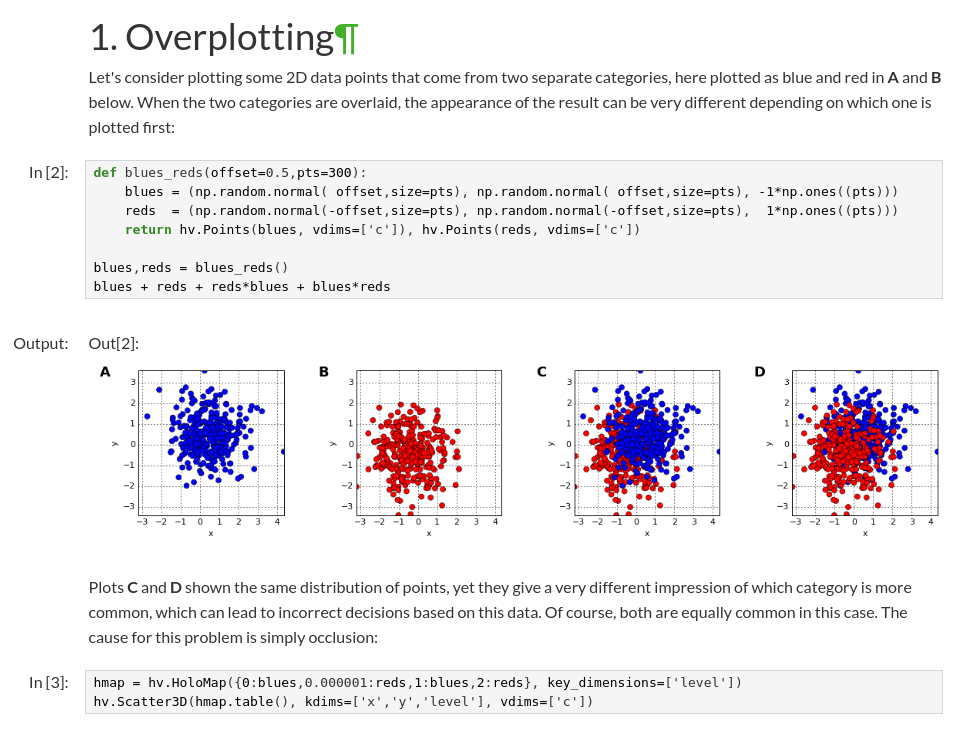
\includegraphics[width=\textwidth]{ipython}
  \caption{A plot from data in an IPython notebook.}
  \label{fig:ipython}
\end{figure}

As explained, IPython and Jupyter notebooks have become more or less separate
projects, to the extent that Jupyter notebooks can use several kernels.
Nowadays there are kernels for over 40 languages that can be used in these
notebooks. This illustrates that in Python's case literate programming is more
or less an extension to the interactive IPython REPL. Since Jupyter notebooks
reuse the IPython REPL, the execution model used for Jupyter notebooks is
essentially the same as it is for IPython~\cite{ipython-execution}.

%%% Local Variables:
%%% mode: latex
%%% TeX-master: "main"
%%% End:


\section{Problem Definition}
\label{sec:a-problem-definition}

The previous sections provided the necessary background knowledge of
the problem domain. Now that the background knowledge has been
explained, this section will discuss the problem definition of the
client.

Spoofax offers a wide variety of tools to develop DSLs and
accompanying IDE support. Precisely because Spoofax is concerned with
developing DSLs, rapid prototyping of syntax and grammar is a
convenient addition to the product. \Cref{sec:a-repl} showed that REPLs
provide this rapid prototyping ability for other languages like Lisp
and Python. Therefore, the client has expressed their interest in
a REPL that works with all language definitions created in
Spoofax. Such a REPL would aid both the developer of the language and
its end-user.

Since a lot of language services are already provided by Spoofax, the
REPL should try to hook into existing services as much as possible.
Besides exposing already existing Spoofax services in a REPL,
the product should also expose additional features geared
towards interactive exploration of programs in Spoofax defined
languages.  Examples include displaying and editing the contents of
current program context, saving and loading program context and
keeping a history of executed expressions.

When a REPL is realized in time, the product could be further extended to add
support for literate programming, allowing for rapid prototyping and
documentation at the same time~\cite{schulte2012}. This would allow
developers of new DSLs to document and explain their language in an
interactive manner that directly allows experimentation.

%%% Local Variables:
%%% mode: latex
%%% TeX-master: "main"
%%% End:


\section{Problem Analysis}
\label{sec:problem-analysis}
This section gives an analysis of the problem as defined in the
previous section \ref{sec:problem-definition}. More specifically, this
section describes the problems that are expected and to be solved
during the implementation process of the product. The first part of
this section describes the process of incorporating REPL generation
within the larger context of Spoofax. The second part analyzes the
part of the problem concerned with literate programming, but this part
will be analyzed in less detail than generating REPLs as it is unsure
whether this will be present in the final product.

\subsection{Incorporating REPL generation within Spoofax}
\label{ssec:incorp-repl-gener}
To generate solidly working REPLs for any language defined in Spoofax,
some Spoofax concepts have to be carefully considered. Since every
language can have many different language constructs, generating REPLs
should not be constrained to language specific constructs like
classes, but should rather be done generically. Therefore the
implementation and particularly the interaction with the user needs to
be thought of carefully.

This section lists the problems that are expected when trying to
implement generating REPLs generically. For each problem, their
solution approaches that should be explored during the implementation
process are given, as well as the parts of Spoofax that are relevant
for that problem.

\subsubsection{Redefining the contents bound to names}
\label{sec:redef-cont-bound}
% TODO: Is "content" the right terminology here?
\todo{FIXME: Just noting possible solutions we might want to elaborate}
We could add ...
\begin{itemize}
\item a special prefix for shell specific commands, and then...
\item a command to enumerate all possible namespaces as detected by spoofax
\item a command to switch to a namespace from this list
\item a command to list entries in the current namespace
\item expressions typed will be added to the selected namespace
\item all language agnostic, since we won't care what to call the namespace
\end{itemize}

\subsubsection{Detecting unfinished expressions for multiline editing}
\label{sec:detect-unfin-expr}

\subsection{Extending the product with literate programming}
\label{sec:extend-prod-with}

\subsection{Plug-in development in Eclipse}
\label{ssec:eclipse-plugins}

%%% Local Variables:
%%% mode: latex
%%% TeX-master: "main"
%%% End:


\section{Requirements Analysis}
\label{sec:requirement-analysis}

Defining requirements upfront is important for several reasons: it is a contract
between the developers and the client, it guides the product development, it
enables the client to track the progress and finally it allows validation of the
deliverable. These requirements are listed in this section.

\subsection{Design goals}
\label{ssec:goals}

The client has expressed some high-level requirements, which are listed in this
subsection as design goals in order of priority. The design goals serve as an
important guideline when defining and implement the invidual requirements. As
such, they can be considered the bounds within which all requirements must fit.

\paragraph{Language-agnostic} A REPL should be generated for each language
defined with Spoofax. This means that no assumptions can be made about any
language constructs or syntax.

\paragraph{Autogeneration} The REPLs should be automatically generated, just
like all of Spoofax's other services. This means that generating a shell should
be integrated into Spoofax's build system and should not require any additional
steps from the user.

\paragraph{Maintainability} Spoofax is an already existing, open source project
managed by several people. When the product is delivered, it will have to be
maintained by others. Therefore, it is important that the code is maintainable.

\paragraph{Performance} Spoofax's developers already focus quite a bit on
performance: both the generation and the use of the services are performant.
This should be no different for the generation and use of the REPL.

\paragraph{Modify Spoofax's existing codebase as little as possible} The product
should be an extension to Spoofax, which means the changes made to the existing
Spoofax codebase should be as small as possible. Preferably, the REPL service
generator should be a standalone module.

\subsection{Requirements}
\label{ssec:requirements}

Under the guidance of the design goals listed in the previous subsection, the
requirements compiled from the feature matrix discussed in \cref{sec:repl} and
meetings with the client are discussed below, under the MoSCoW method.

\subsubsection{Must have}

Requirements listed under ``must haves'' are of critical importance to the
usability and success of the deliverable. Without these, the product is not in a
workable state and is not likely to be accepted by the client. \emph{Must} can
also be considered an acronym for the Minimum Usable SubseT.

\paragraph{Interactive shell} Per the definition of a REPL given in
\cref{sec:repl}, the generated REPLs have to be interactive. It should evaluate
single statements and expressions typed in by the user and print the results
back to them.

\paragraph{Generated from language definition} Every service generated by
Spoofax is made from the language definitions. It is evident that the REPL
should be generated from the same definitions if it is to fit within Spoofax.

\paragraph{Input \& output history} Users should be able to retrieve previously
typed expressions and statements to support the explorative and interactive
nature of a REPL. In the same vein, previously yielded results should be
implicitly bound to automatically generated names to make their values available
in future expressions.

\paragraph{Multiline input editing} Most, if not all, modern languages benefit
by structuring their constructs over multine lines. Multiline input editing is
therefore a crucial feature for user satisfaction. The input editor should
start in single line editing mode and recognise when an expression or statement
is part of a multiline construction. When it recognises this, it should
automatically switch to its multiline input editing mode, wherein the
prompt character indicates this new mode. This mode's behavior (e.g. keyboard
shortcuts) is different from the single line editing mode.

\paragraph{Error reporting} To support the interactivity of the REPL, error
reporting should be available in two ways: while typing an expression or a
statement, on-the-fly error reporting should indicate wrongly typed items. The
interpreter that evaluates syntactically correct input should also be able to
display its error messages to the user in case of an error during the dynamic
semantics phase.

\paragraph{Syntax checked input} Supporting the above requirement, all
input should have its syntax checked on the fly.

\paragraph{Syntax highlighting} All expressions and statements (whether they are
currently being entered, displayed as previously entered input or displayed as
previously yieled results) should be syntax highlighted.

\paragraph{Integration with Eclipse} As first implementation, the generated
REPLs should integrate with Eclipse to provide an interface to the users. It is
important to note that while integration with Eclipse is a requirement, Spoofax
itself is moving to be IDE-agnostic. As such, the implementation of the REPL's
core should be generic and should not be tied to Eclipse.

\subsubsection{Should have}

Requirements listed under ``should-haves'' are important, but not necessary for
a working product.

\paragraph{Ability to redefine identifiers} As explained in \cref{sec:repl},
REPLs provide the ability to explore unknown problem domains. It is not a
far-fetched idea that a developer would want to change function implementations
or the types of certain variables. To support this, a REPL should allow users to
redefine identifiers. This might mean that the REPL needs different semantics
than the language it operates on, slightly contrasting the requirement that the
REPLs should be language-agnostic.

\paragraph{Environment inspection} The argument of the previous requirements can
be repeated for this one: the exploratory and interactive nature of REPLs call
for the ability to inspect the current environment. This is to replace the files
with source code that a developer could otherwise inspect and an initial step
towards offering debugging features in a REPL.

\paragraph{Save and load shell state} Often, developers want to save the current
state of their IDE and return to it later. As such, the REPLs should allow their
state to be saved and restored.

\subsubsection{Could have}

Requirements listed under ``could-haves'' are desirable, but not necessary.
These requirements often improve usability or customer satisfaction and are
included only if time permits.

\paragraph{Context-sensitive code completion} The multiline input editor should
ideally function just like an IDE's editor. Context-sensitive code completion is
therefore a nice feature to offer the users. Context-sensitive code-completion
also helps with the discoverability of APIs and therefore is another step
towards the explorative and interactive environment a REPL is supposed to
provide.

\paragraph{Hover over variables to see value, type and others} Another step
towards debugging would be the ability to hover variables with the mouse in
order to inspect their value, type and other known information. The difference
between this feature and the previously mentioned environment inspection is that
this feature works per variable.

\paragraph{Literate programming} As explained in
\cref{sec:literate-programming}, literate programming offers the advantage that
code and documentation go hand in hand. This allows developers of languages in
Spoofax to document and illustrate their language simultaneously with the
development: documentation and examples can never be outdated, because outdated
example code will halt the execution.

\paragraph{Integration with other IDEs (IntelliJ)} As mentioned before, Spoofax
is currently undergoing a transition not to be tied to a specific IDE.
Generation of Spoofax's editor services to IntelliJ are currently a work in
progress and it would be nice if the generated REPLs work in IntelliJ from the
start.

\subsubsection{Won't have}

Requirements listed under ``won't-haves'' are not for implementation in this
project. They have been identified as possible features, but are outside of the
scope of this project and listed only as possible suggestions for further work.

\paragraph{GDB-style debugging and nested REPLs} Spoofax currently does not
generate any debugging features, which would be required for REPLs to offer such
functionality as a built-in feature. Writing such debugging generators is
outside the scope of this project and as such, offering debugging capabilities
inside the REPLs is something to consider for a later version.

\subsection{Minimal viable product}
\label{ssec:mvp}

The design goals and requirements listed in the previous subsections give a good
idea of what the deliverable should look like. It is possible, however, that due
to unforeseen problems, not all the listed requirements and design goals can be
met. It is important to therefore define a minimal subset of the design goals
and requirements that \emph{must} be present in the final deliverable: the
``must have'' requirements have to be implemented, whilst adhering to the first
two design goals.

%%% Local Variables:
%%% mode: latex
%%% TeX-master: "main"
%%% End:


\section{Frameworks and Tools}
\label{sec:a-realisation-product}

The previous section analyzed the requirements for the product as set in
\cref{sec:a-requirement-analysis}. The purpose of this section is to discuss the
frameworks and tools used during the development of the product.

\subsection{Development frameworks}
\label{ssec:a-frameworks}

Spoofax is an already existing project. In order for the product to be as easily
integrated as possible, most of the tooling used by Spoofax will be reused. This
means that the Java programming language is to be used, together with Maven for
the build environment and JUnit for unit tests. On top of this, Spoofax uses a
few open source Java libraries as can be seen in the list below. It is most
likely that these will be used in the product as well.

The only exception to this is the fact that TravisCI is used as opposed to
Jenkins, because Jenkins is self-hosted whilst TravisCI is available for free
online.

\begin{itemize}
  \item Guice, a lightweight dependency injection framework;
  \item Guava, provides general utilities missing in the JDK;
  \item RxJava, a library for composing asynchronous and event-based programs
    using observable sequences;
  \item Apache VFS, a library for accessing various different file systems;
  \item EhCache, a standards-based cache that boosts performance;
  \item Apache's logging library.
\end{itemize}

If new libraries are to be used during the development of the project, it is
important that these are under a license compatible with the Apache license
under which Spoofax is licensed. Compatible licenses include, but are not
limited to, the LGPL, MIT, BSD and Apache licenses.

\subsection{Development tools}
\label{ssec:a-tools}

To manage the source code, the git version control system is used. Pull-based
development~\cite{Gousios14} is the paradigm chosen, in order for each member of
the team to work on their assigned tasks without interfering with each other.
To facilitate this, the GitHub platform is used because if offers an easy
interface to pull-based development: it automatically discovers the commits to
be merged, it facilitaties code review and discussion, new commits are
automatically added to the pull-request so that the discussion can continue and
GitHub automatically verifies whether commits can be merged. On top of this,
GitHub also provides an integrated issue tracker.

Furthermore, the tools FindBugs and PMD will be used to assist in delivering
quality code. Checkstyle will be used to guarantee a coherent style throughout
the code. These three static analysis tools will help ensure the design goal of
maintainability, as highlighted in \cref{ssec:a-goals}.

%%% Local Variables:
%%% mode: latex
%%% TeX-master: "main"
%%% End:


\section{Conclusion}
\label{sec:conclusion}

The purpose of this research report was to explore the problem domain, to define
and analyse the problem which the product is to resolve and to analyse its
requirements.

The first three sections explored the problem domain; the Spoofax Language
Workbench, read-eval-print loops and literate programming were investigated.
These three separate domains come together when working towards a viable product.

The next section defined the problem, which is to bring rapid prototyping and
exploratory programming to users who are defining programming languages in
Spoofax. This problem was then analyzed in the following section, wherein it
was outlined how the product will fit into the existing Spoofax codebase.
Several issues were foreseen and discussed together with possible solutions.
From the problem definition and analysis, a list of requirements was compiled.
These requirements are structured using the MoSCoW method. The ``must-haves'',
together with outlined design goals, form a minimal viable product. Finally,
the last section discussed the development frameworks and tools to be used.

With the research phase now complete, an overview has been formed as to what the
product should do and how it should be implemented.

%%% Local Variables:
%%% mode: latex
%%% TeX-master: "main"
%%% End:


\appendix

\bibliography{references}{}

%% Comment out for glossaries
%\glossarystyle{altlistgroup}
%\printglossaries{}

\end{document}

%%% Local Variables:
%%% mode: latex
%%% TeX-master: t
%%% End:
